\chapter{Modelos de Regresión Bayesianos}

Parafraseando a \textcite{DraperSmith98}, al realizar un análisis estadístico sobre algún fenómeno que presenta variabilidad, muchas veces lo que se busca es explorar los efectos que algunas \textit{variables explicativas} ejercen--- o parecen ejercer--- sobre una \textit{variable de interés}. En algunos casos puede darse que, efectivamente, exista una relación funcional simple entre ambos tipos de variables. No obstante es mucho más común que, o bien la relación sea mucho más compleja de lo que podemos entender o describir, o bien simplemente nos es desconocida. En ambos casos, lo que podemos hacer es \textit{modelar}--- esto es, aproximar--- la relación mediante algunas funciones matemáticas. Por razones históricas relacionadas con el trabajo de Sir Francis Galton esta clase de modelos se conocen como \textit{modelos de regresión} \parencite{Zepeda15}. 

\section{Regresión lineal} 
 
En el caso más sencillo, tendríamos que $y=f(x)$. Sin embargo, en la mayoría de los casos este modelo tomado literalmente podría parecernos una mala aproximación. Pensemos en el caso en el que se busca describir el peso en kilogramos de una persona a partir de la estatura. Es claro que a una misma estatura le podrían corresponder distintos valores de peso. A pesar de ello, podemos observar empíricamente que a mayor estatura \textit{esperamos} un mayor peso. Esto nos llevaría a pensar que podemos modelar el \textit{valor esperado} de nuestra variable de interés mediante alguna función de las variables explicativas.\\

Esto quiere decir que, bajo una perspectiva bayesiana paramétrica, modelaremos la incertidumbre sobre la variable de interés $Y$ mediante una distribución de probabilidad condicional $f(y|\theta,x)$. Las variables explicativas $X$ determinan esta distribución condicional a través del valor esperado mediante una función que depende también de un subconjunto de parámetros $\theta_d$: 
\begin{equation} \label{eq:regr_gral}
Y|\theta,X \sim f(y|\theta,x) \qquad \E{Y|\theta,X} = h(\theta_d,X)
\end{equation} 
Las formas más simples de la función $h(\theta_d,X)$ son \textit{lineales en los coeficientes}, esto es de la forma siguiente 
\begin{equation*}
h(\theta_d,X) = \beta_0 + \beta_1X_1 + \beta_2X_2 + \dots + \beta_{d-1}X_{d-1}, 
\end{equation*}
para $d-1$ variables explicativas y donde $\theta_d = (\beta_0,\beta_1,\dots,\beta_{d-1})$. El vector general de parámetros $\theta$ entonces se descompone en dos--- $\theta = (\theta_d,\theta_r)$--- con $\theta_r$ posibles parámetros adicionales de la distribución condicional de $Y$ dado $X$ pero que no determinan su esperanza. Las variables explicativas pueden llegar a ser transformaciones unas de otras como cuando se buscan ajustar relaciones de orden cuadrático o como cuando se incluyen interacciones.\\

Debido a que no conocemos la verdadera relación entre nuestras variables, tenemos incertidumbre sobre los valores de los coeficientes que determinan nuestra función $h(\theta_d ,X)$ y, posiblemente, sobre el resto de parámetros $\theta_r$. Así pues, bajo la perspectiva bayesiana debemos reflejar dicha incertidumbre también mediante alguna distribución de probabilidad $f(\theta)$. Buscaremos, entonces, reducirla mediante la recolección de datos $(y,x)$ que nos permitan, a través del teorema de Bayes obtener la distribución posterior $f(\theta|y,x)$.\\

Como bien notan tanto \textcite{Gelman13} como \textcite{Congdon06}, el modelo más general debería incorporar también la incertidumbre que pudiera existir sobre las variables explicativas $X$ derivada, por ejemplo, de posibles errores de medición. Sin embargo, si se puede asumir que los parámetros $\varphi$ de la distribución de $X$, $f(x|\varphi)$, son independientes de $\theta$--- es decir $f(\varphi,\theta)=f(\varphi)f(\theta)$--- al aplicar el Teorema de Bayes veríamos que la distribución posterior $f(\theta|y,x)$ no dependería de $\varphi$ por lo que podemos proceder ignorando dicha incertidumbre para efectos de las inferencias sobre $\theta$. Por eso--- y para simplificar la notación--- a partir de aquí omitiré la condicional en $X$, con lo que $f(\theta|y,x)$ se convierte en $f(\theta|y)$, por ejemplo. \\

El modelo de regresión más usual es cuando se asume que la variable de interés se distribuye normal con una media que depende linealmente de las variables explicativas. Esto es, supongamos que tenemos $N$ conjuntos de observaciones, condicionalmente independientes, $\left\lbrace(y_i,x_{i,1},\dots,x_{i,d-1})\right\rbrace_{i=1}^{N}$ donde nuestra variable de interés es $Y$ y contamos con $d-1$ variables explicativas $\left\lbrace X_j\right\rbrace_{j=1}^{d-1}$, la regresión lineal normal bajo los supuestos usuales es: 
\begin{align*} 
y_i = \beta_0 + \beta_1 x_{i,1} + \dots + \beta_{d-1} x_{i,d-1} + \epsilon_i \qquad \epsilon_i \sim N(0,\sigma^2) \quad \forall i = 1,\dots, N. 
\end{align*}
Que en términos de \eqref{eq:regr_gral} sería
\begin{equation*}
y_i|\theta \sim N(\mu_i,\sigma^2) \quad \mu_i = \E{y_i|\theta} = \beta x_i \quad \forall i = 1, \dots, N,
\end{equation*}
donde $\beta = (\beta_0,\beta_1,\dots,\beta_{d-1})$, $x_i = (1,x_{i,1},\dots,x_{i,d-1})$ y tal que  $\theta = (\beta,\sigma^2)$ tenga alguna distribución inicial apropiada.\\ 

También es posible aprovechar la notación matricial para simplificar estas expresiones, así como trabajar con ellas. Definiendo lo siguiente,  
\begin{align*}
X &= 
\begin{pmatrix}
  1 & x_{1,1} & \cdots & x_{1,d-1} \\
  \vdots & \vdots & \ddots & \vdots  \\
  1 & x_{N,1} & \cdots & x_{N,d-1} 
\end{pmatrix} \in \mathbb{R}_{N\mathsf{x}d}, \\
y &= (y_1,\dots,y_N)^T \in \mathbb{R}_{N\mathsf{x}1},\\
\beta &= (\beta_0,\beta_1,\dots,\beta_{d-1})^T \in \mathbb{R}_{d\mathsf{x}1}, 
\end{align*}
tenemos que el modelo de regresión normal puede ser expresado de manera compacta de la siguiente forma: 
\begin{equation*}
y|\theta \sim N_N(X\beta,\sigma^2\mathbb{I}_N) \quad \text{tal que} \quad \theta = (\beta, \sigma^2) \sim f(\beta,\sigma^2), 
\end{equation*} 
donde $N_N(X\beta,\sigma^2\mathbb{I}_N)$ representa una distribución normal $N-$variada con media $X\beta$ y varianzas individuales $\sigma^2$ y $f(\beta,\sigma^2)$ una distribución inicial para los parámetros desconocidos. 

\subsection{Problema de multicolinealidad} \label{prob_multicolinealidad}

Antes de continuar, debo señalar un posible problema cuando uno ajusta modelos de regresión. En el \textbf{Anexo \ref{Anexo_modelo_lineal}} se muestra el desarrollo del modelo lineal normal utilizando iniciales conjugadas--- que pueden ser informativas o débilmente informativas--- así como un caso límite que resulta ser la inicial no informativa de Jeffreys. El estimador máximo verosimil $b=(X^TX)^{-1}X^Ty$ es clave para el análisis. En dicho desarrollo asumo que es posible calcular $b$, aún cuando no siempre es el caso.\\

El estimador involucra la matriz inversa $(X^TX)^{-1}$, pero no siempre es posible invertir una matriz. Para ello se requiere que todas sus columnas sean lo que en álgebra lineal se conoce como \textit{linealmente independientes}. Esto no pasa si hay variables explicativas tales que exista una combinación lineal de ellas que sea igual a $0$ para todos los datos \parencite{GelmanHill06}. Cuando esto sucede se dice que dichas variables son linealmente dependientes o bien que son \textit{colineales}.\\

El caso más sencillo de colinealidad es cuando se utiliza una variable categórica $X$ a través de su representación como variables indicadoras. Esto quiere decir que si $X$ tiene $J$ categorías, podemos representarla como un vector de $J$ variables diferentes $X \equiv (X_1,X_2,\dots,X_J)$. Cuando $X$ toma el valor de la $j$-ésima categoría, todas las variables del vector son iguales a $0$ y solamente hay un $1$ en la correspondiente a la categoría de la observación: $(X_1 = 0,\dots,X_j = 1,\dots,X_J=0)$. Así, la suma de las $J$ variables dicotómicas siempre es igual a $1$. El problema se materializa cuando consideramos que el intercepto en una regresión es equivalente a una variable explicativa ficticia igual a $1$, por lo que al restarle la suma de las $J$ variables dicotómicas se obtiene una combinación lineal de variables explicativas igual a $0$ para todos los datos, i.e. dependencia lineal.\\ 

Una forma de evitar el problema es excluyendo el término del intercepto en la regresión. Sin embargo, si existe una segunda variable categórica, el problema se repite. Para resolverlo, entonces, se tienen que incorporar restricciones. Una de las más frecuentes es la llamada restricción de esquina \parencite{Regueiro12}. Esta consiste en obligar a uno de los coeficientes de las categorías a que tome el valor de $0$, lo que equivale a excluir una de las $J$ categorías y solo incorporar $J-1$ variables dicotómicas. Cuando la variable toma el valor de la categoría excluida, el vector de las $J-1$ restantes es un vector de ceros. Así, si existen otras variables categóricas, se puede proceder de la misma manera escogiendo, para cada una de ellas, una categoría de referencia para excluir \parencite{GelmanHill06}.\\ 

Otra solución consiste en imponer una restricción de tipo suma cero. En este caso el valor de uno de los coeficientes se fija como el negativo de la suma del resto de los coeficientes de las variables linealmente dependientes:
\begin{equation*}
\beta_j=-\sum\limits_{k\neq j}\beta_k.
\end{equation*}
Esta restricción tiene como consecuencia que los efectos de las diferentes categorías no pueden ser todos positivos o todos negativos \parencite{Usi14}.\\

Ahora bien, en términos estadísticos normalmente se habla del problema de \textit{multicolinealidad} porque incluso si no hay colinealidad exacta, hay ocasiones que los datos están altamente correlacionados y esto tiene como consecuencia que sea difícil invertir la matriz $X^TX$ \parencite{Usi14}. Una manera de atacar este problema es agregar información que permita facilitar la inversión, por ejemplo a través de la distribución inicial \parencite{Congdon06}.\\ 


\section{Modelos Lineales Generalizados}

El modelo lineal normal es muy flexible--- sobre todo aprovechando que puede construirse en términos de variables transformadas--- pero, hay ocasiones en las que pudiera no ser el más adecuado. Por ejemplo, cuando la variable tiene restricciones pudiera no ser posible utilizar la regresión normal, incluso mediante una transformación, como cuando una variable no negativa puede tomar el valor de $0$ y entonces aplicar el logaritmo no funciona \parencite{Gelman13}. Este caso se presenta con frecuencia en el estudio de fenómenos políticos relacionados con el voto, pues es posible que el número de votos sea realmente $0$. De manera similar, si se estudian proporciones de votos, estas toman valores entre $0$ y $1$ lo que puede dificultar la aplicación del modelo tradicional que tiene soporte en todos los números reales. Cuando la variable de interés representa conteos, podría también dificultarse la aplicación del modelo lineal.\\ 

En estos casos existen otras alternativas de modelado. Una familia más general de modelos de regresión son los modelos lineales generalizados, mismos que consituyen un marco teórico general y unificado para pensar en la formulación de modelos estadísticos \parencites{Dobson01}. Antes de introducirlos, sin embargo, necesitamos una definición dada por \textcite{Nieto16} y que es un caso particular de la que utilizaron \textcite{NelderWedderburn72} al presentar originalmente esta clase de modelos. 

\dfn{\textbf{Familia Exponencial}\\
\label{def:Fam_Exp}
Sea $Y$ una variable aleatoria con función de distribución $f\left(y|\theta, \phi \right)$ tal que 
\begin{equation} \label{eq:fam_exp}
f\left(y|\theta,\phi\right) = b(y,\phi)exp\left\lbrace\phi\left[y\theta-a(\theta)\right]\right\rbrace,
\end{equation}
donde $a$ y $b$ son funciones conocidas. Se dice entonces que $Y$ pertenece a la \textbf{familia exponencial}. Cuando el parámetro de dispersión $\phi$ es conocido, entonces $Y$ pertenece a la \textbf{familia exponencial natural}.\\
}

Esta familia de distribuciones incluye a las más comunes, como la Normal, la Poisson o la Bernoulli \parencite{Nieto16}. Con este tipo de distribuciones construimos los modelos lineales generalizados. Como se verá en la definición que sigue, la idea informal de la sección anterior también está presente en ellos. En efecto, los modelos lineales generalizados nos permitirán modelar una variable aleatoria de interés mediante una distribución condicional miembro de la familia exponencial, vinculando su valor esperado con las variables explicativas.

\dfn{\textbf{Modelo lineal generalizado} (MLG)\\
\label{def:MLG}
Un modelo lineal generalizado, abreviado \textbf{MLG}, está compuesto por 3 elementos básicos: 

\begin{enumerate}
\item \textbf{Variable aleatoria de interés}: se supone que la variable de interés $Y$ se distribuye condicionalmente de acuerdo a alguna ley miembro de la familia exponencial. Esto es, $f(y|\theta,\phi)$ es alguna distribución de la forma de \eqref{eq:fam_exp}.
\begin{equation*}
Y|\theta,\phi \sim f(y|\theta,\phi) = b(y,\phi)exp\left\lbrace\phi\left[y\theta-a(\theta)\right]\right\rbrace.
\end{equation*}
A este elemento se le conoce también como \textit{componente aleatoria}.
\item \textbf{Predictor lineal}: las variables explicativas $X$ forman un predictor lineal en los coeficientes de la forma $\eta=X\beta$. Esto es, suponiendo que tenemos $d-1$ variables explicativas $X$ e incluyendo quizás a un intercepto constante:
\begin{equation*}
\eta=X\beta=\beta_0 + \beta_1X_1 + \dots + \beta_{d-1}X_{d-1}.
\end{equation*}
Este elemento es llamado también \textit{componente sistemática}.
\item \textbf{Función liga}: el predictor lineal se vincula con nuestra variable de interés mediante una función liga invertible $g(\cdot)$. La forma específica del vínculo es que el valor del predictor lineal es el resultado de aplicar la función liga al valor esperado condicional de la variable de interés. Esto es, sea $\mu$ el valor esperado de $Y|\theta,\phi$, entonces 
\begin{equation*}
g(\mu) = \eta = X\beta.
\end{equation*}
Otra forma de ver la función liga es que el valor esperado de $Y|\theta,\phi$ es el resultado de aplicar al predictor lineal la función inversa de la liga: 
\begin{equation*}
\mu = g^{-1}(\eta) = g^{-1}(X\beta).
\end{equation*}
\end{enumerate}

Bajo el paradigma bayesiano, además, un MLG debe incluir un cuarto elemento que refleje la incertidumbre existente sobre los parámetros del modelo: 

\begin{enumerate}
\setcounter{enumi}{3}
\item \textbf{Distribución Inicial}: la incertidumbre o el conocimiento incial que se tenga sobre los parámetros $\theta$ y, en su defecto $\phi$, se refleja en una distribución inicial de probabilidad $f(\theta,\phi)$. Nótese que en un MLG los parámetros $\theta$ de la variable de interés, incluyen a los coeficientes $\beta$ del predictor lineal.
\end{enumerate}
}
 
En lo que sigue, me referiré a $N$ observaciones de una variable de interés $Y$, condicionalmente independientes dadas $d-1$ variables explicativas, de manera tal que para cada individuo $i\in \mathbb{N}_N$, $y_i$ representaría la observación de la variable de interés, $X_i = (1, x_{i,\,1}, \dots ,x_{i,\,d-1})$ el correspondiente vector de variables explicativas y $\beta=(\beta_0, \beta_1, \dots, \beta_{d-1})^T$ el vector de coeficientes del predictor lineal.

\subsubsection*{Modelo Normal}

El modelo usual de regresión lineal para variables de interés continuas en los reales puede expresarse como MLG de la siguiente manera: 
\begin{align*}
y_i|\beta,\sigma^2 & \sim N(\mu_i,\sigma^2) \quad \forall \quad i \in \mathbb{N}_N \nonumber \\
\text{con} \quad \mu_i &= X_i\beta \nonumber \\
\beta,\sigma^2 &\sim f(\beta,\sigma^2)
\end{align*}
En este caso tenemos que la función liga resulta ser la identidad, lo que se conoce como \textit{liga canónica}. 

\subsubsection*{Modelo Poisson}

Cuando nuestra variable de interés representa conteos, un modelo usual es la regresión Poisson o loglineal, en el que la liga resulta ser el logaritmo natural. En este caso el parámetro de dispersión $\phi$ no está presente; dicho de otra forma $\phi=1$, por lo que la distribución Poisson es un caso de una distribución exponencial natural. 
\begin{align*}
y_i|\beta & \sim Poi(\lambda_i) \quad \forall \quad i \in \mathbb{N}_N \nonumber \\
\text{con} \quad log(\lambda_i) &= X_i\beta \nonumber \\
\beta &\sim p(\beta)
\end{align*}

\subsection{Regresión logística}\label{Sec:Pres_Logis}

A continuación presento con más detalle uno de los MLG más conocidos y utilizados: la regresión logística. Esta busca modelar $f(y|\theta)$ mediante una distribución Bernoulli. La relación entre las variables explicativas y el valor esperado se construye con un predictor lineal para el logit de la probabilidad de éxito del ensayo de Bernoulli. Es decir, si $p = \Pr(Y=1)$ es la probabilidad de éxito, entonces $log\left(\dfrac{p}{1-p}\right)=X\beta$.\\ 

En otras ocasiones, nuestra variable de interés podría ser binomial, es decir, los éxitos en una serie de ensayos Bernoulli independientes. Para cada observación $y_i$, además de las variables explicativas, conocemos también $n_i$, el número de ensayos Bernoulli para el $i$-ésimo individuo. Es decir, es posible generalizar una regresión logística para que el número de ensayos sea mayor a $1$. Veamos ahora cómo construir el modelo como un MLG.

\subsubsection*{Modelo Binomial}

En primer lugar debemos probar que una variable binomial, con parámetro $n$ conocido, puede expresarse como miembro de la familia exponencial. 
\begin{align*}
Y|p \sim Binom(n,p) \;\Leftrightarrow\; f(y|p) &= {n\choose y}p^y(1-p)^{n-y} \\
\;\Leftrightarrow\; f(y|p) &= {n\choose y}\,exp\left\lbrace log\left[p^y(1-p)^{n-y}\right]\right\rbrace \\
\;\Leftrightarrow\; f(y|p) &= {n\choose y}\,exp\left\lbrace y\,log\left(\dfrac{p}{1-p}\right)+n\,log\left(1-p\right)\right\rbrace
\end{align*}
Definiendo el logit de $p$ como nuestro parámetro $\theta$, tenemos que $\theta = log\left(\dfrac{p}{1-p}\right)$ y al despejar $p = \dfrac{e^\theta}{1+e^\theta}$, por lo que podemos podemos sustituir: \begin{align} \label{eq:Veros_Binomial}
\Rightarrow f(y|p) &= {n\choose y}\,exp\left\lbrace y\,\theta+n\,log\left(1-\dfrac{e^\theta}{1+e^\theta}\right)\right\rbrace \nonumber \\
&= {n\choose y}\,exp\left\lbrace y\,\theta+n\,log\left(\dfrac{1}{1+e^\theta}\right)\right\rbrace \nonumber \\
&= {n\choose y}\,exp\left\lbrace y\,\theta-n\,log\left(1+e^\theta\right)\right\rbrace
\end{align} 
Así, tenemos que una variable binomial con parámetro $n$ conocido se expresa de la forma de \eqref{eq:fam_exp} tomando los siguientes valores: 
\begin{align*}
\theta &= log\left(\dfrac{p}{1-p}\right) \qquad \phi = 1\\
a(\theta) &= n\,log\left(1+e^\theta\right) \qquad b(\theta,y) = {n\choose y}
\end{align*}
Ahora bien, habiendo ilustrado la pertenencia a la familia exponencial, el MLG binomial normalmente se plantea en términos de $p_i$, el valor esperado de cada uno de los ensayos de Bernouilli \parencite{Gelman13}:
\begin{align*}
Y_i|\beta & \sim Binom(n_i,p_i) \quad \forall \quad i \in \mathbb{N}_N \nonumber \\
\text{con} \quad log\left(\dfrac{p_i}{1-p_i}\right) &= X_i\beta \nonumber \\
\beta &\sim f(\beta)
\end{align*}
En este caso, debido a que cada valor esperado binomial $\mu_i$ es igual a $n_ip_i$, tenemos que $p_i=\mu_i/n_i$. Por lo que la tradicional función logística implícitamente refleja la siguiente función liga: 
\begin{align*}
log\left(\dfrac{p_i}{1-p_i}\right)&=log(p_i)-log(1-p_i)\\
&=log\left(\dfrac{\mu_i}{n_i}\right)-log\left(1-\dfrac{\mu_i}{n_i}\right)\\ 
&= log\left(\dfrac{\mu_i}{n_i}\right)-log\left(\dfrac{n_i-\mu_i}{n_i}\right)\\
&=log\left(\mu_i\right)-log\left(n_i-\mu_i\right)\\ 
\therefore \quad g(\mu_i)&=log\left(\dfrac{\mu_i}{n_i-\mu_i}\right)
\end{align*}

\subsubsection{Problema analítico} \label{sec:Prob_Analitico}

Ahora supongamos que queremos realizar un análisis bayesiano y actualizar nuestras creencias mediante el teorema de Bayes. Podríamos llevarnos la desagradable sorpresa de que una regresión logística no tiene las mismas facilidades analíticas que sí tiene el modelo normal del \textbf{Anexo \ref{Anexo_modelo_lineal}}. De manera particular, no podemos encontrar una distribución conjugada.\\ 

En efecto, definiendo $\theta_i = log\left(\dfrac{p_i}{1-p_i}\right)=X_i\beta$ y utilizando la forma de la función de verosimilitud en \eqref{eq:Veros_Binomial}, donde $y$ representa el vector de observaciones de nuestra variable de interés: 
\begin{align} \label{eq:Veros_Binomial_MLG} 
f(y|\beta) &= f(y_1,\dots,y_N|\beta)= \prod_{i=1}^N f(y_i|\beta) \nonumber\\
&= \prod_{i=1}^N {n_i\choose y_i}\,exp\left\lbrace y_i\,X_i\beta-n_i\,log\left(1+e^{X_i\beta}\right)\right\rbrace \nonumber\\
&\propto \prod_{i=1}^N exp\left\lbrace y_i\,X_i\beta-n_i\,log\left(1+e^{X_i\beta}\right)\right\rbrace \nonumber\\
&\propto exp\left\lbrace \sum\limits_{i=1}^Ny_i\,X_i\beta-n_i\,log\left(1+e^{X_i\beta}\right)\right\rbrace 
\end{align}
Esta no es una forma funcional que permita encontrar fácilmente una inicial conjugada conocida.\\

En el mismo sentido, supongamos que tomamos como iniciales independientes para los coeficientes, distribuciones normales centradas en $0$ con cierta desviación estándar común $\sigma$, conocida. Veamos cómo luce la actualización de la verosimilitud en \eqref{eq:Veros_Binomial_MLG} por esta inicial normal multivariada: 
\begin{align*}
f(y|\beta) &\propto exp\left\lbrace \sum\limits_{i=1}^N y_i\,X_i\beta-n_i\,log\left(1+e^{X_i\beta}\right)\right\rbrace \\
&\propto exp\left\lbrace (\beta yX)^T-\sum\limits_{i=1}^Nn_i\,log\left(1+e^{X_i\beta}\right)\right\rbrace; \\
f(\beta) &= \dfrac{1}{\sqrt{(2\pi)|\sigma^2 \mathbb{I}_N|}}exp\left\lbrace -\dfrac{1}{2}\beta^T(\sigma^2\mathbb{I}_N)^{-1}\beta\right\rbrace \\
&\propto exp\left\lbrace -\dfrac{\beta^T\beta}{2\sigma^2}\right\rbrace, \\
\Rightarrow \; f(\beta|y)&\propto f(y|\beta)f(\beta) \\
&\propto exp\left\lbrace -\dfrac{\beta^T\beta}{2\sigma^2} + (\beta yX)^T-\sum\limits_{i=1}^Nn_i\,log\left(1+e^{X_i\beta}\right)\right\rbrace \\
&\propto exp\left\lbrace -\dfrac{1}{2\sigma^2}\left[\beta^T\beta - 2\sigma^2(\beta yX)^T\right]\right\rbrace\prod_{i=1}^N \left(1+e^{X_i\beta}\right)^{-n_i}
\end{align*}

Esta expresión tampoco permite un tratamiento analítico bajo una forma funcional conocida. No es posible integrarla para conocer la constante de normalización y así tener completa la distribución posterior.\\

¿Acaso es posible llevar a cabo una simple regresión logística bajo el paradigma bayesiano? Por mucho tiempo la respuesta a esta pregunta era prácticamente no. Como la integral no se puede calcular, la alternativa es obtenerla mediante aproximaciones analíticas como la llamada \textit{aproximación de Laplace} o bien mediante integración numérica mediante métodos de cuadratura \parencites{Nieto16,GP97}. Sin embargo, estos métodos son muy difíciles de aplicar cuando la dimensión del problema empieza a crecer.\\ 

Afortunadamente, el desarrollo de las computadoras permitió superar este obstáculo y, desde la década de 1990, el paradigma bayesiano ha ido creciendo con fuerza. Hoy es posible aplicar modelos como la regresión logística y más complejos sin problemas. Por ello, pospongo el tema de cómo calcular las integrales al \textbf{\autoref{chap:Cap_MCMC}} y continúo con la discusión general de los modelos de regresión. 

\section{Modelos Jerárquicos}

Los modelos de regresión--- ya sean lineales o lineales generalizados--- pueden interpretarse como un método que permite aproximar cómo cambia el valor esperado de una variable de interés a través de subpoblaciones definidas por funciones lineales de unas variables explicativas \parencite{GelmanHill06}. En efecto, podemos pensar que diferentes valores de las variables explicativas definen diferentes subpoblaciones o grupos cuyos valores promedio en la variable de interés está determinado por la regresión. A pesar de esta variabilidad, la \textit{forma específica} como cambian estos valores es la misma a través de las subpoblaciones pues está dada por los mismos coeficientes. De manera informal, podemos decir que las observaciones de todas las subpoblaciones tienen cierta simetría que las hace similares entre sí a nuestros ojos y por eso comparten los mismos parámetros.\\ 

No obstante, hay ocasiones en las que dicha simetría es más débil o, mejor dicho, podemos distinguir claramente subpoblaciones o grupos de observaciones como más homogéneas al interior que entre sí. Es decir, la simetría la encontramos para observaciones provenientes de la misma subpoblación y no entre aquellas que pertenezcan a grupos distintos. El ejemplo más claro es cuando, por diseño, nuestro estudio está compuesto por estratos de observaciones.\\ 

Uno esperaría mayor homogeneidad de los resultados en algún examen entre estudiantes de una misma escuela que entre aquellos de diferentes instituciones educativas \parencite{Ortiz12}; de la misma manera, cuando se busca estimar el resultado de una elección con base en encuestas publicadas habrían más diferencias entre encuestas de diferentes casas que entre ejercicios de la misma organización \parencite{Zepeda18}. En la práctica, este razonamiento implica que no queremos tratar a las distintas subpoblaciones o grupos con la misma cuchara y, por tanto, deben tener distintos parámetros o coeficientes; por ejemplo, cuando los efectos estacionales en la prevalencia de una enfermedad son distintos para diferentes regiones geográficas \parencite{Usi14}.\\ 

Una primera posibilidad es mantener una sola regresión incluyendo variables indicadoras de pertenencia al grupo. Sin embargo, este camino puede fallar incluso en situaciones más o menos sencillas. ¿Qué pasa si se tienen variables explicativas a nivel grupo? No es posible incluir al mismo tiempo tanto estas variables como las indicadoras pues tendríamos un problema de multicolinealidad \parencite{GelmanHill06}. Otra alternativa es ajustar regresiones separadas para cada grupo. Sin embargo, el hecho de que se traten de \textit{subpoblaciones} y no de \textit{poblaciones} o fenómenos completamente distintos nos haría pensar que si bien los parámetros son diferentes, deben estar de todas formas relacionados. Más aún, ajustar regresiones separadas a cada grupo tiene el defecto de que cada una de ellas incorpora exclusivamente la información del grupo respectivo, desperdiciando de alguna manera la información sobre el fenómeno o población general que los datos de las otras subpoblaciones pueden aportar.\\

Así pues, tenemos dos extremos que pudieran no parecernos ideales. Por un lado, podemos pensar que todos los datos son similares entre sí y, por tanto, ajustamos una sola regresión. Esta opción sería una \textit{agrupación completa} o \textit{complete-pooling}. El costo de tomar este camino podría ser subestimar la variabilidad originada por las diferentes subpoblaciones debido a que estamos sobresimplificando el modelo asumiendo la simetría total. En el otro extremo, podríamos suponer que cada subpoblación es completamente distinta y se requieren tantas regresiones independientes como grupos hayan. Un modelo así sería \textit{sin agrupación} o de \textit{no-pooling}. En este caso, un riesgo que corremos es que las estimaciones podrían ser demasiado ruidosas o inciertas debido a que estarían ignorando la información sobre la población general que comparten las observaciones de las distintas subpoblaciones o por el simple hecho de que hayan muy pocas observaciones por grupo, por ejemplo.\\ 

Existe otra alternativa conocida como modelos jerárquicos o multinivel y que representan un punto intermedio entre las dos anteriores mediante una \textit{agrupación parcial} de los datos o \textit{partial-pooling}. Su objetivo es reconocer las diferencias que existen a través de diferentes subpoblaciones mediante una estructura jerárquica que incorpore la información de todas ellas con relación a la población general.

\subsection{Intercambiabilidad}

Los modelos jerárquicos tienen su piedra angular en el concepto de intercambiabilidad que es la formalización de la idea de simetría u homogeneidad en los datos de la que hablaba. Su definición está basada en la de \textcite{BernardoSmith00}.\\ 

\dfn{\textbf{Intercambiabilidad}\\
\label{def:Intercambiabilidad}
Sean $X_1,\dots,X_n$ una sucesión finita de variables aleatorias. Se dice que son \textbf{finitamente intercambiables} si y solo si, para toda permutación $\pi$ definida sobre el conjunto de índices $\mathbb{N}_n$, su distribución conjunta satisface que 
\begin{equation*}
f(X_1 = x_1, \dots, X_n = x_n) = f(X_1 = x_{\pi(1)},\dots, X_n = x_{\pi(n)}).
\end{equation*}
La sucesión infinita $X_1,X_2,\dots$ es \textbf{infinitamente intercambiable} si y solo si toda subsucesión finita es finitamente intercambiable.\\ 
}

Cuando asumimos que unas variables aleatorias son independientes, se cumple la propiedad de intercambiabilidad, pero el concepto de intercambiabilidad es un poco más general; queremos decir que los índices o etiquetas de las observaciones pueden cambiar y no los distinguiríamos. Para comprobar que independencia implica intercambiabilidad basta observar que, si hay independencia, la distribución conjunta se descompone en un producto y ``el orden de los factores no altera el resultado". Sin embargo, no es cierto que intercambiabilidad implique independencia, como puede verse en el contraejemplo de \textcite{GP98}. En este caso es natural asumir una representación de independencia condicional dado un parámetro común para las observaciones.\\ 

Dicha \textit{naturalidad} puede justificarse a partir de un caso particular del Teorema de representación de De Finetti que establece que la densidad conjunta de unas variables aleatorias intercambiables puede representarse mediante el uso de la independencia condicional dado un parámetro: 
\begin{equation*}
f(x_1,\dots,x_n) = \int\limits_\Theta \prod\limits_{i=1}^n f(x_i|\theta)f(\theta)d\theta.
\end{equation*} 
El lector interesado puede consultar \textcite{GP98} o \textcite{BernardoSmith00}.\\ 

Cabe aclarar que la condición de intercambiabilidad que supone el Teorema de representación de De Finetti es de intercambiabilidad infinita, pero normalmente al modelar tratamos con observables que más bien satisfarían solamente una intercambiabilidad finita. A pesar de esto, si se da el caso en el que la secuencia finita de variables aleatorias observadas pueda representar una parte de una secuencia más larga de variables finitamente intercambiables, es posible asumir intercambiabilidad infinita como una aproximación suficientemente buena y proceder en consecuencia \parencite{BernardoSmith00}. Este es el supuesto, a veces tácito, que normalmente se hace en un modelo estadístico \parencite{Gelman13}.\\

\begin{figure}[h]
	\centering
	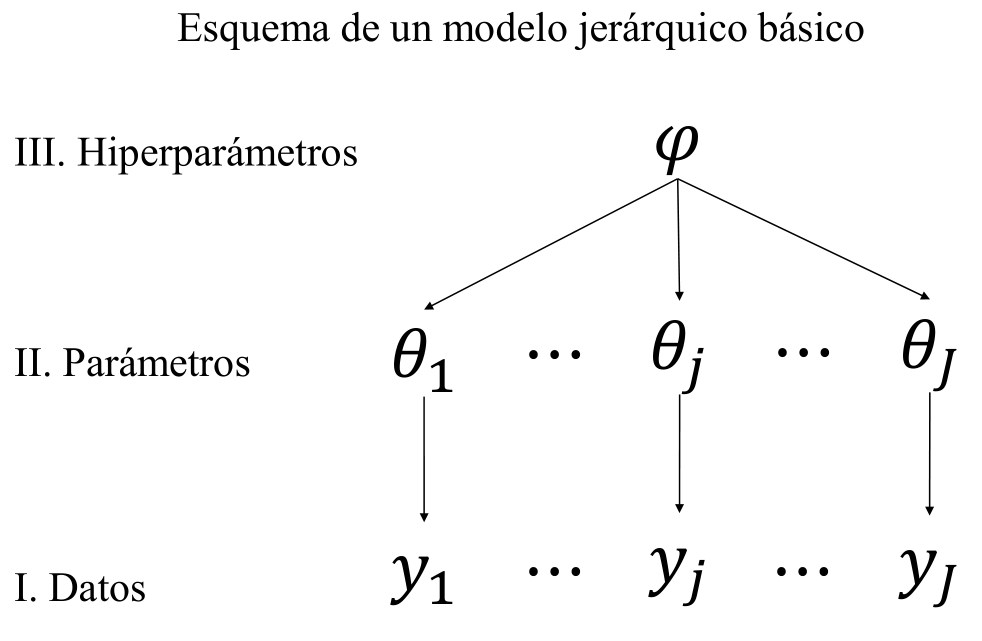
\includegraphics[scale=0.25]{Figs/Bayes/Modelo_Jer}
	\caption{Esquema de un modelo jerárquico básico para $J$ subpoblaciones. Los datos de cada subpoblación $y_j$ son condicionalmente independientes dado un parámetro $\theta_j$. Los parámetros $\theta$ son, a su vez, intercambiables y se modelan condicionalmente independientes dado un hiperparámetro poblacional $\varphi$. Fuente: elaboración propia.}
	\label{fig:Esquema_Modelo_Jer}	
\end{figure}

Ahora bien, un modelo jerárquico establece la intercambiabilidad de las observaciones al interior de cada subpoblación mediante la independencia condicional dado un parámetro grupal. Esto haría también un modelo de no agregación, mientras que una agregación completa asume esto para toda la población. Lo que distingue a un modelo jerárquico es que adicionalmente supone intercambiabilidad para los parámetros de cada grupo de manera que estos sean condicionalmente independientes dado uno o más \textit{hiperparámetros} poblacionales. Esto puede verse de manera esquemática en la \textbf{Figura \ref{fig:Esquema_Modelo_Jer}}, mientras que en términos de las distribuciones del modelo tendríamos los siguientes niveles: 
\begin{align*}
&\text{I Datos} \quad & f(y|\theta)&=f(y_1,\dots,y_J|\theta_1,\dots,\theta_J)=\prod\limits_{j=1}^Jf(y_j|\theta_j) \\
&\text{II Parámetros} \quad & f(\theta|\varphi)&=f(\theta_1,\dots,\theta_J|\varphi) = \prod\limits_{j=1}^Jf(\theta_j|\varphi)  \\
&\text{III Hiperparámetros} \quad & f(\varphi)&
\end{align*}

Un modelo jerárquico aumenta el número de parámetros a estimar al agregar los hiperparámetros. Entonces, tenemos que la distribución inicial de los parámetros depende de un hiperparámetro mismo que, para realizar el aprendizaje bayesiano, deberá tener una distribución \textit{hiperinicial}. El problema consiste en inferir tanto las características de las subpoblaciones, $\theta_j$, como aquellas poblacionales, $\varphi$ \parencite{GP98}: 
\begin{align*}
f(\theta,\varphi|y) & \propto f(y|\theta,\varphi)f(\theta,\varphi) \\
&\propto f(y|\theta)f(\theta|\varphi)f(\varphi) \\
&\propto f(\varphi)\prod\limits_{j=1}^Jf(y_j|\theta_j)\prod\limits_{j=1}^Jf(\theta_j|\varphi) \\
&\propto f(\varphi)\prod\limits_{j=1}^Jf(y_j|\theta_j)f(\theta_j|\varphi)
\end{align*}

\subsection{Regresiones jerárquicas}

En términos de regresiones, los modelos jerárquicos son aquellos en los que los coeficientes también son modelados mediante hiperparámetros estimados con los mismos datos \parencite{GelmanHill06}. Esto permite pensar en regresiones a distintos niveles y con variables grupales, estudios con base en muestreo estratificado e incluso estructuras no necesariamente anidadas. Las ventajas de los modelos jerárquicos hacen que, para algunos investigadores, las regresiones multinivel merezcan ser el enfoque predeterminado \parencite{McElreath15}.\\

De manera general es posible clasificar las regresiones jerárquicas en tres grandes categorías: interceptos variables, pendientes variables e interceptos y pendientes variables. De manera gráfica estos pueden verse en la \textbf{Figura \ref{fig:Ejemplos_Jer}}. Para presentarlas, supongamos que tenemos $N$ observaciones $\left\lbrace(y_i,x_i,u_{j[i]})\right\rbrace_{i=1}^{N}$ agrupadas en $J$ grupos. Nuestra variable de interés es $Y$, contamos con una variable explicativa a nivel individuo, $X$,  y una a nivel grupo,  $U$.  Debido a que ahora tenemos $J$ grupos, indico con la notación $j[i]$ el grupo al que pertenece el $i$-ésimo individuo. En el \textbf{Cuadro \ref{tbl:Regr_Jer_Lineales}} presento ejemplos esquemáticos de este tipo para modelos lineales en los que $\alpha$ representa el intercepto y $\beta$ la pendiente de la recta; en el caso de los \textit{hipercoeficientes} estos se representan por $a$ y $b$.\\

\begin{figure}[h]
    \centering
    \begin{subfigure}{0.3\textwidth}
        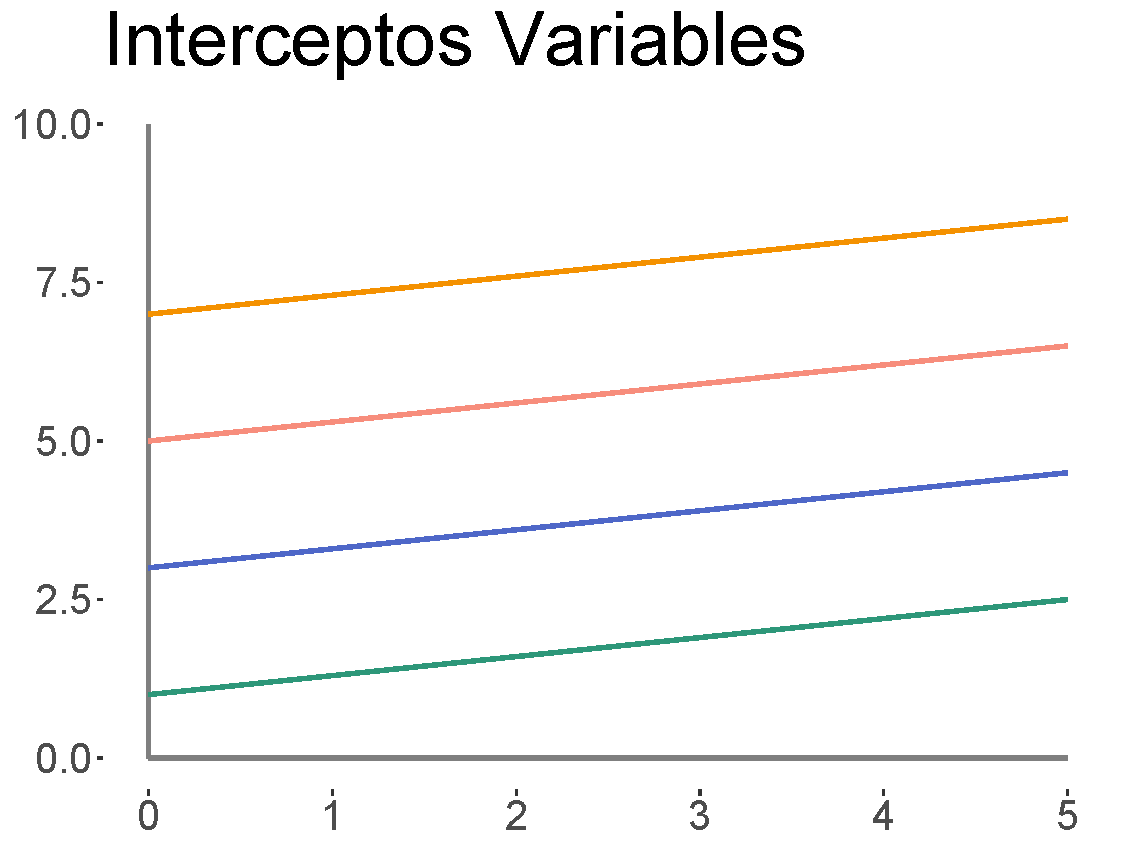
\includegraphics[width=\textwidth]{Figs/Bayes/Interceptos_Variables}
        \label{fig:Ejemplos_Jer_Int_Var}
        \caption{$y_i = \alpha_{j[i]} + \beta x_i$}
    \end{subfigure}
    ~ 
    \begin{subfigure}{0.3\textwidth}
        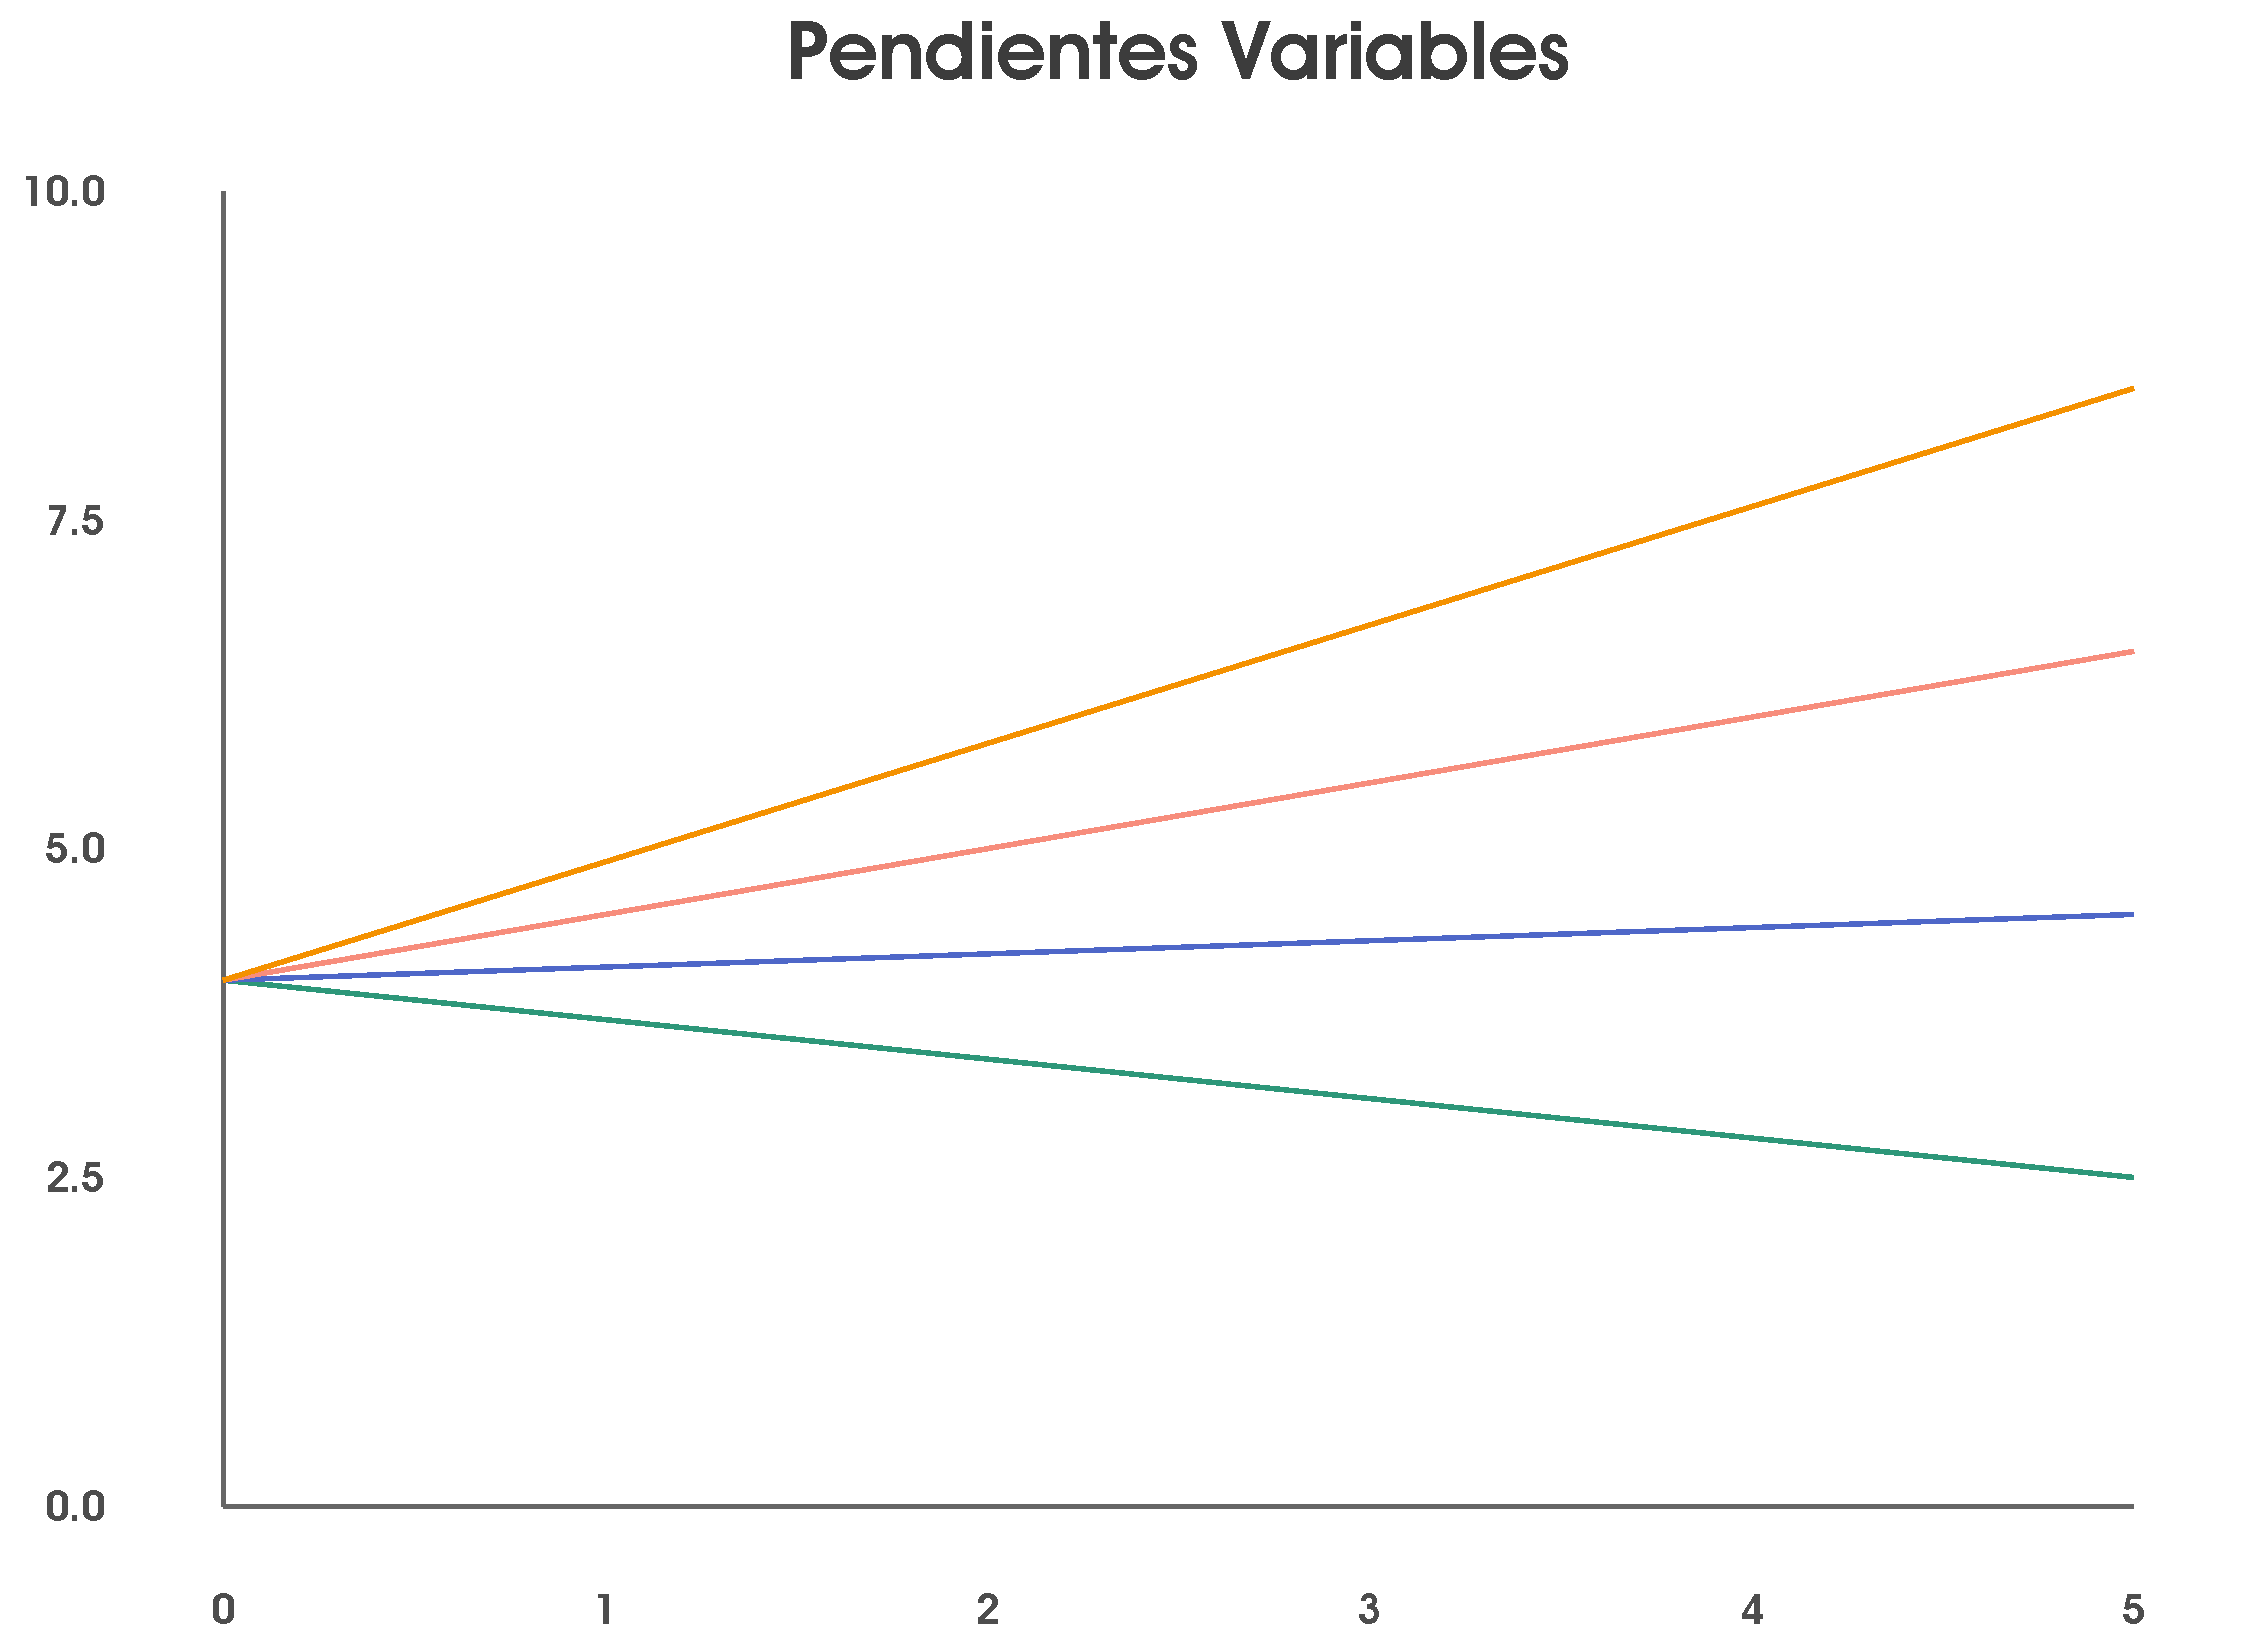
\includegraphics[width=\textwidth]{Figs/Bayes/Pendientes_Variables}
        \label{fig:Ejemplos_Jer_Pend_Var}
        \caption{$y_i = \alpha + \beta_{j[i]} x_i$}
    \end{subfigure}
    ~
    \begin{subfigure}{0.3\textwidth}
        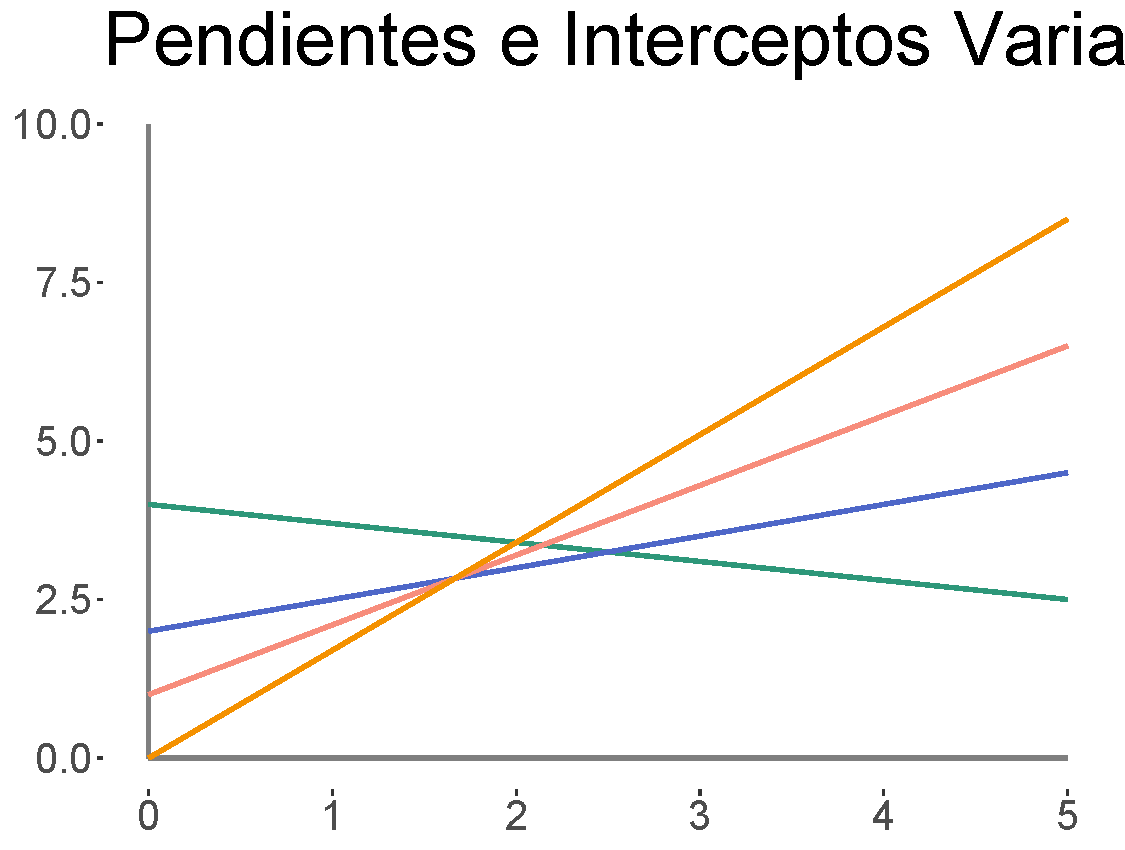
\includegraphics[width=\textwidth]{Figs/Bayes/Pend_e_Inter_Variables}
        \label{fig:Ejemplos_Jer_Pend_Int_Var}
        \caption{$y_i = \alpha_{j[i]} + \beta_{j[i]} x_i$}
    \end{subfigure}
    \caption{Ilustración de los tres tipos generales de modelos jerárquicos. Fuente: elaboración propia con base en la figura (11.1) de \textcite{GelmanHill06}.}\label{fig:Ejemplos_Jer}
\end{figure}

Una de las ventajas que tienen los modelos jerárquicos es que cuando se tiene una variable categórica--- a diferencia de lo que sucede en un modelo lineal normal (ver página \pageref{prob_multicolinealidad})--- no es necesario excluir una categoría de referencia. Por el contrario, es posible conservar el intercepto y todas las variables indicadoras dicotómicas con sus respectivos coeficientes. La clave está en que los coeficientes ahora tienen a su vez una distribución que los modela, misma que tiene el efecto de agregar un término a la matriz $X^TX$, lo que la convierte en una matriz invertible y elimina este caso particular de multicolinealidad \parencite{GelmanHill06}. 

\begin{table}
\centering
\resizebox{\linewidth}{!}{
\begin{tabular}{l l l l}
Nivel de jerarquía & \textbf{Interceptos variables} & \textbf{Pendientes variables} & \textbf{Interceptos y pendientes variables} \\
\hline 
\\
I. Datos & 
	$\;y_i \sim N(\alpha_{j[i]} + \beta x_i,\sigma_y^2)$ & 
	$\;y_i \sim N(\alpha + \beta_{j[i]} x_i,\sigma_y^2)$ &
	$\;y_i \sim N(\alpha_{j[i]} + \beta_{j[i]} x_i,\sigma_y^2)$\\ 
	\\
	\\
II. Parámetros & 
	$\;\alpha_{j[i]} \sim N(a + b u_{j[i]}, \sigma_{\alpha}^2)$ & 
	$\;\beta_{j[i]} \sim N(a + b u_{j[i]}, \sigma_{\beta}^2)$ &
	$\;\alpha_{j[i]} \sim N(a_{\alpha} + b_{\alpha} u_{j[i]}, \sigma_{\alpha}^2)$\\
	\\[-1ex] 
	& 
	& 
	&
	$\;\beta_{j[i]} \sim N(a_{\beta} + b_{\beta} u_{j[i]}, \sigma_{\beta}^2)$ \\
	\\
	\\
III. Hiperparámetros & 
	$\;f(\varphi) = f(\beta,\sigma_y^2,a,b,\sigma_{\alpha}^2)$ & 
	$\;f(\varphi) = f(\alpha,\sigma_y^2,a,b,\sigma_{\beta}^2)$ &
	$\;f(\varphi) = f(\sigma_y^2,a_{\alpha},b_{\alpha},\sigma_{\alpha}^2,a_{\beta},b_{\beta},\sigma_{\beta}^2)$\\
\end{tabular}}
\caption{Ejemplos esquemáticos de regresiones jerárquicas lineales. Fuente: elaboración propia.}
\label{tbl:Regr_Jer_Lineales}
\end{table}


\subsubsection*{Regresión logística jerárquica}

Naturalmente, es posible proponer MLG jerárquicos. Por ejemplo, una regresión logística jerárquica con algunas \textit{hiperiniciales} arbitrarias sería la siguiente: 
\begin{align*}
y_i|\alpha_{j[i]},\beta_{j[i]} & \sim Binom(n_i,p_i) \\
log\left(\dfrac{p_i}{1-p_i}\right) &= \alpha_{j[i]} + \beta_{j[i]} x_i  \\ 
\alpha_{j[i]} & \sim N(a_{\alpha} + b_{\alpha} u_{j[i]}, \sigma_{\alpha}^2) \\ 
\beta_{j[i]} & \sim N(a_{\beta} + b_{\beta} u_{j[i]}, \sigma_{\beta}^2) \\ 
a_{\alpha} \sim N(0,5) & \quad  a_{\beta} \sim N(0,5) \\
b_{\alpha} \sim N(0,5) & \quad  b_{\beta} \sim N(0,5) 
\end{align*}

Como puede intuirse, la estructura de un modelo jerárquico crece rápidamente. Sin embargo, recordemos que la \textit{única receta de la inferencia bayesiana} sigue siendo la misma: encontrar la distribución condicional de todas aquellas cantidades de interés cuyo valor desconocemos, dado el valor conocido de las variables observadas. Gracias a herramientas computacionales este cálculo es posible para modelos cada vez más complejos. En el siguiente capítulo, entonces, discutiré algunos métodos computacionales que permiten este aprendizaje bayesiano. 
